\documentclass[1p]{elsarticle_modified}
%\bibliographystyle{elsarticle-num}

%\usepackage[colorlinks]{hyperref}
%\usepackage{abbrmath_seonhwa} %\Abb, \Ascr, \Acal ,\Abf, \Afrak
\usepackage{amsfonts}
\usepackage{amssymb}
\usepackage{amsmath}
\usepackage{amsthm}
\usepackage{scalefnt}
\usepackage{amsbsy}
\usepackage{kotex}
\usepackage{caption}
\usepackage{subfig}
\usepackage{color}
\usepackage{graphicx}
\usepackage{xcolor} %% white, black, red, green, blue, cyan, magenta, yellow
\usepackage{float}
\usepackage{setspace}
\usepackage{hyperref}

\usepackage{tikz}
\usetikzlibrary{arrows}

\usepackage{multirow}
\usepackage{array} % fixed length table
\usepackage{hhline}

%%%%%%%%%%%%%%%%%%%%%
\makeatletter
\renewcommand*\env@matrix[1][\arraystretch]{%
	\edef\arraystretch{#1}%
	\hskip -\arraycolsep
	\let\@ifnextchar\new@ifnextchar
	\array{*\c@MaxMatrixCols c}}
\makeatother %https://tex.stackexchange.com/questions/14071/how-can-i-increase-the-line-spacing-in-a-matrix
%%%%%%%%%%%%%%%

\usepackage[normalem]{ulem}

\newcommand{\msout}[1]{\ifmmode\text{\sout{\ensuremath{#1}}}\else\sout{#1}\fi}
%SOURCE: \msout is \stkout macro in https://tex.stackexchange.com/questions/20609/strikeout-in-math-mode

\newcommand{\cancel}[1]{
	\ifmmode
	{\color{red}\msout{#1}}
	\else
	{\color{red}\sout{#1}}
	\fi
}

\newcommand{\add}[1]{
	{\color{blue}\uwave{#1}}
}

\newcommand{\replace}[2]{
	\ifmmode
	{\color{red}\msout{#1}}{\color{blue}\uwave{#2}}
	\else
	{\color{red}\sout{#1}}{\color{blue}\uwave{#2}}
	\fi
}

\newcommand{\Sol}{\mathcal{S}} %segment
\newcommand{\D}{D} %diagram
\newcommand{\A}{\mathcal{A}} %arc


%%%%%%%%%%%%%%%%%%%%%%%%%%%%%5 test

\def\sl{\operatorname{\textup{SL}}(2,\Cbb)}
\def\psl{\operatorname{\textup{PSL}}(2,\Cbb)}
\def\quan{\mkern 1mu \triangleright \mkern 1mu}

\theoremstyle{definition}
\newtheorem{thm}{Theorem}[section]
\newtheorem{prop}[thm]{Proposition}
\newtheorem{lem}[thm]{Lemma}
\newtheorem{ques}[thm]{Question}
\newtheorem{cor}[thm]{Corollary}
\newtheorem{defn}[thm]{Definition}
\newtheorem{exam}[thm]{Example}
\newtheorem{rmk}[thm]{Remark}
\newtheorem{alg}[thm]{Algorithm}

\newcommand{\I}{\sqrt{-1}}
\begin{document}

%\begin{frontmatter}
%
%\title{Boundary parabolic representations of knots up to 8 crossings}
%
%%% Group authors per affiliation:
%\author{Yunhi Cho} 
%\address{Department of Mathematics, University of Seoul, Seoul, Korea}
%\ead{yhcho@uos.ac.kr}
%
%
%\author{Seonhwa Kim} %\fnref{s_kim}}
%\address{Center for Geometry and Physics, Institute for Basic Science, Pohang, 37673, Korea}
%\ead{ryeona17@ibs.re.kr}
%
%\author{Hyuk Kim}
%\address{Department of Mathematical Sciences, Seoul National University, Seoul 08826, Korea}
%\ead{hyukkim@snu.ac.kr}
%
%\author{Seokbeom Yoon}
%\address{Department of Mathematical Sciences, Seoul National University, Seoul, 08826,  Korea}
%\ead{sbyoon15@snu.ac.kr}
%
%\begin{abstract}
%We find all boundary parabolic representation of knots up to 8 crossings.
%
%\end{abstract}
%\begin{keyword}
%    \MSC[2010] 57M25 
%\end{keyword}
%
%\end{frontmatter}

%\linenumbers
%\tableofcontents
%
\newcommand\colored[1]{\textcolor{white}{\rule[-0.35ex]{0.8em}{1.4ex}}\kern-0.8em\color{red} #1}%
%\newcommand\colored[1]{\textcolor{white}{ #1}\kern-2.17ex	\textcolor{white}{ #1}\kern-1.81ex	\textcolor{white}{ #1}\kern-2.15ex\color{red}#1	}

{\Large $\underline{12n_{0635}~(K12n_{0635})}$}

\setlength{\tabcolsep}{10pt}
\renewcommand{\arraystretch}{1.6}
\vspace{1cm}\begin{tabular}{m{100pt}>{\centering\arraybackslash}m{274pt}}
\multirow{5}{120pt}{
	\centering
	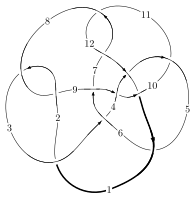
\includegraphics[width=112pt]{../../../GIT/diagram.site/Diagrams/png/2724_12n_0635.png}\\
\ \ \ A knot diagram\footnotemark}&
\allowdisplaybreaks
\textbf{Linearized knot diagam} \\
\cline{2-2}
 &
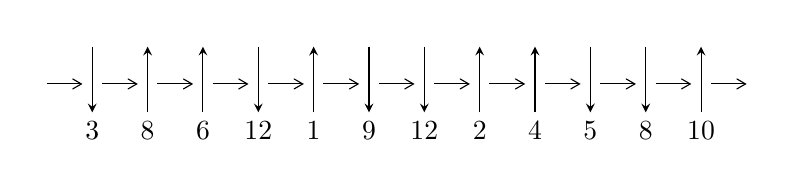
\begin{tikzpicture}[x=20pt, y=17pt]
	% nodes
	\node (C0) at (0, 0) {};
	\node (C1) at (1, 0) {};
	\node (C1U) at (1, +1) {};
	\node (C1D) at (1, -1) {3};

	\node (C2) at (2, 0) {};
	\node (C2U) at (2, +1) {};
	\node (C2D) at (2, -1) {8};

	\node (C3) at (3, 0) {};
	\node (C3U) at (3, +1) {};
	\node (C3D) at (3, -1) {6};

	\node (C4) at (4, 0) {};
	\node (C4U) at (4, +1) {};
	\node (C4D) at (4, -1) {12};

	\node (C5) at (5, 0) {};
	\node (C5U) at (5, +1) {};
	\node (C5D) at (5, -1) {1};

	\node (C6) at (6, 0) {};
	\node (C6U) at (6, +1) {};
	\node (C6D) at (6, -1) {9};

	\node (C7) at (7, 0) {};
	\node (C7U) at (7, +1) {};
	\node (C7D) at (7, -1) {12};

	\node (C8) at (8, 0) {};
	\node (C8U) at (8, +1) {};
	\node (C8D) at (8, -1) {2};

	\node (C9) at (9, 0) {};
	\node (C9U) at (9, +1) {};
	\node (C9D) at (9, -1) {4};

	\node (C10) at (10, 0) {};
	\node (C10U) at (10, +1) {};
	\node (C10D) at (10, -1) {5};

	\node (C11) at (11, 0) {};
	\node (C11U) at (11, +1) {};
	\node (C11D) at (11, -1) {8};

	\node (C12) at (12, 0) {};
	\node (C12U) at (12, +1) {};
	\node (C12D) at (12, -1) {10};
	\node (C13) at (13, 0) {};

	% arrows
	\draw[->,>={angle 60}]
	(C0) edge (C1) (C1) edge (C2) (C2) edge (C3) (C3) edge (C4) (C4) edge (C5) (C5) edge (C6) (C6) edge (C7) (C7) edge (C8) (C8) edge (C9) (C9) edge (C10) (C10) edge (C11) (C11) edge (C12) (C12) edge (C13) ;	\draw[->,>=stealth]
	(C1U) edge (C1D) (C2D) edge (C2U) (C3D) edge (C3U) (C4U) edge (C4D) (C5D) edge (C5U) (C6U) edge (C6D) (C7U) edge (C7D) (C8D) edge (C8U) (C9D) edge (C9U) (C10U) edge (C10D) (C11U) edge (C11D) (C12D) edge (C12U) ;
	\end{tikzpicture} \\
\hhline{~~} \\& 
\textbf{Solving Sequence} \\ \cline{2-2} 
 &
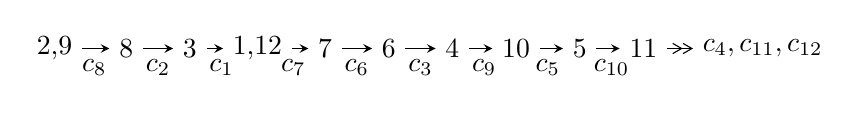
\begin{tikzpicture}[x=23pt, y=7pt]
	% node
	\node (A0) at (-1/8, 0) {2,9};
	\node (A1) at (1, 0) {8};
	\node (A2) at (2, 0) {3};
	\node (A3) at (49/16, 0) {1,12};
	\node (A4) at (33/8, 0) {7};
	\node (A5) at (41/8, 0) {6};
	\node (A6) at (49/8, 0) {4};
	\node (A7) at (57/8, 0) {10};
	\node (A8) at (65/8, 0) {5};
	\node (A9) at (73/8, 0) {11};
	\node (C1) at (1/2, -1) {$c_{8}$};
	\node (C2) at (3/2, -1) {$c_{2}$};
	\node (C3) at (5/2, -1) {$c_{1}$};
	\node (C4) at (29/8, -1) {$c_{7}$};
	\node (C5) at (37/8, -1) {$c_{6}$};
	\node (C6) at (45/8, -1) {$c_{3}$};
	\node (C7) at (53/8, -1) {$c_{9}$};
	\node (C8) at (61/8, -1) {$c_{5}$};
	\node (C9) at (69/8, -1) {$c_{10}$};
	\node (A10) at (11, 0) {$c_{4},c_{11},c_{12}$};

	% edge
	\draw[->,>=stealth]	
	(A0) edge (A1) (A1) edge (A2) (A2) edge (A3) (A3) edge (A4) (A4) edge (A5) (A5) edge (A6) (A6) edge (A7) (A7) edge (A8) (A8) edge (A9) ;
	\draw[->>,>={angle 60}]	
	(A9) edge (A10);
\end{tikzpicture} \\ 

\end{tabular} \\

\footnotetext{
The image of knot diagram is generated by the software ``\textbf{Draw programme}" developed by Andrew Bartholomew(\url{http://www.layer8.co.uk/maths/draw/index.htm\#Running-draw}), where we modified some parts for our purpose(\url{https://github.com/CATsTAILs/LinksPainter}).
}\phantom \\ \newline 
\centering \textbf{Ideals for irreducible components\footnotemark of $X_{\text{par}}$} 
 
\begin{align*}
I^u_{1}&=\langle 
7.72790\times10^{299} u^{118}-1.72629\times10^{299} u^{117}+\cdots+2.99648\times10^{300} b-1.21626\times10^{302},\\
\phantom{I^u_{1}}&\phantom{= \langle  }-5.20063\times10^{302} u^{118}-4.63209\times10^{302} u^{117}+\cdots+6.32257\times10^{302} a-1.43930\times10^{305},\\
\phantom{I^u_{1}}&\phantom{= \langle  }u^{119}+u^{118}+\cdots-366 u+211\rangle \\
I^u_{2}&=\langle 
-144442009874 u^{40}-40660630315 u^{39}+\cdots+55254454982 b+95137731796,\\
\phantom{I^u_{2}}&\phantom{= \langle  }-121324231307 u^{40}-226756643017 u^{39}+\cdots+55254454982 a-930709060133,\\
\phantom{I^u_{2}}&\phantom{= \langle  }u^{41}+11 u^{39}+\cdots+3 u+1\rangle \\
\\
\end{align*}
\raggedright * 2 irreducible components of $\dim_{\mathbb{C}}=0$, with total 160 representations.\\
\footnotetext{All coefficients of polynomials are rational numbers. But the coefficients are sometimes approximated in decimal forms when there is not enough margin.}
\newpage
\renewcommand{\arraystretch}{1}
\centering \section*{I. $I^u_{1}= \langle 7.73\times10^{299} u^{118}-1.73\times10^{299} u^{117}+\cdots+3.00\times10^{300} b-1.22\times10^{302},\;-5.20\times10^{302} u^{118}-4.63\times10^{302} u^{117}+\cdots+6.32\times10^{302} a-1.44\times10^{305},\;u^{119}+u^{118}+\cdots-366 u+211 \rangle$}
\flushleft \textbf{(i) Arc colorings}\\
\begin{tabular}{m{7pt} m{180pt} m{7pt} m{180pt} }
\flushright $a_{2}=$&$\begin{pmatrix}0\\u\end{pmatrix}$ \\
\flushright $a_{9}=$&$\begin{pmatrix}1\\0\end{pmatrix}$ \\
\flushright $a_{8}=$&$\begin{pmatrix}1\\u^2\end{pmatrix}$ \\
\flushright $a_{3}=$&$\begin{pmatrix}u\\u^3+u\end{pmatrix}$ \\
\flushright $a_{1}=$&$\begin{pmatrix}u^3\\u^5+u^3+u\end{pmatrix}$ \\
\flushright $a_{12}=$&$\begin{pmatrix}0.822551 u^{118}+0.732629 u^{117}+\cdots-379.214 u+227.644\\-0.257900 u^{118}+0.0576106 u^{117}+\cdots-222.436 u+40.5897\end{pmatrix}$ \\
\flushright $a_{7}=$&$\begin{pmatrix}-0.401146 u^{118}+0.0348358 u^{117}+\cdots-399.134 u+76.2959\\-0.243493 u^{118}-0.192213 u^{117}+\cdots+48.6316 u-49.8415\end{pmatrix}$ \\
\flushright $a_{6}=$&$\begin{pmatrix}-0.644639 u^{118}-0.157377 u^{117}+\cdots-350.502 u+26.4544\\-0.243493 u^{118}-0.192213 u^{117}+\cdots+48.6316 u-49.8415\end{pmatrix}$ \\
\flushright $a_{4}=$&$\begin{pmatrix}-0.598905 u^{118}-0.744143 u^{117}+\cdots+316.390 u-182.264\\0.0505679 u^{118}-0.0114233 u^{117}+\cdots+37.3488 u-6.10829\end{pmatrix}$ \\
\flushright $a_{10}=$&$\begin{pmatrix}-0.670832 u^{118}-0.587891 u^{117}+\cdots+246.350 u-149.706\\0.0873593 u^{118}+0.00245992 u^{117}+\cdots+49.1705 u-4.10884\end{pmatrix}$ \\
\flushright $a_{5}=$&$\begin{pmatrix}-0.534374 u^{118}+0.0140889 u^{117}+\cdots-449.449 u+76.2335\\-0.158683 u^{118}-0.273598 u^{117}+\cdots+202.003 u-89.0966\end{pmatrix}$ \\
\flushright $a_{11}=$&$\begin{pmatrix}-0.890241 u^{118}-0.816127 u^{117}+\cdots+395.180 u-249.260\\0.267839 u^{118}+0.00116646 u^{117}+\cdots+230.932 u-37.2540\end{pmatrix}$\\&\end{tabular}
\flushleft \textbf{(ii) Obstruction class $= -1$}\\~\\
\flushleft \textbf{(iii) Cusp Shapes $= 0.432322 u^{118}-2.26997 u^{117}+\cdots+2494.32 u-733.077$}\\~\\
\newpage\renewcommand{\arraystretch}{1}
\flushleft \textbf{(iv) u-Polynomials at the component}\newline \\
\begin{tabular}{m{50pt}|m{274pt}}
Crossings & \hspace{64pt}u-Polynomials at each crossing \\
\hline $$\begin{aligned}c_{1}\end{aligned}$$&$\begin{aligned}
&u^{119}+59 u^{118}+\cdots-926108 u-44521
\end{aligned}$\\
\hline $$\begin{aligned}c_{2},c_{8}\end{aligned}$$&$\begin{aligned}
&u^{119}+u^{118}+\cdots-366 u+211
\end{aligned}$\\
\hline $$\begin{aligned}c_{3}\end{aligned}$$&$\begin{aligned}
&u^{119}-12 u^{118}+\cdots-594 u-503
\end{aligned}$\\
\hline $$\begin{aligned}c_{4}\end{aligned}$$&$\begin{aligned}
&u^{119}+3 u^{118}+\cdots+95214 u-3293
\end{aligned}$\\
\hline $$\begin{aligned}c_{5}\end{aligned}$$&$\begin{aligned}
&u^{119}+u^{118}+\cdots+5201393 u-364301
\end{aligned}$\\
\hline $$\begin{aligned}c_{6}\end{aligned}$$&$\begin{aligned}
&u^{119}-4 u^{118}+\cdots-2916191 u-324667
\end{aligned}$\\
\hline $$\begin{aligned}c_{7},c_{11}\end{aligned}$$&$\begin{aligned}
&u^{119}+u^{118}+\cdots-25 u+1
\end{aligned}$\\
\hline $$\begin{aligned}c_{9}\end{aligned}$$&$\begin{aligned}
&u^{119}+2 u^{118}+\cdots+3981 u+337
\end{aligned}$\\
\hline $$\begin{aligned}c_{10}\end{aligned}$$&$\begin{aligned}
&u^{119}-3 u^{117}+\cdots-14155826 u-953372
\end{aligned}$\\
\hline $$\begin{aligned}c_{12}\end{aligned}$$&$\begin{aligned}
&u^{119}+6 u^{118}+\cdots-6 u-1
\end{aligned}$\\
\hline
\end{tabular}\\~\\
\newpage\renewcommand{\arraystretch}{1}
\flushleft \textbf{(v) Riley Polynomials at the component}\newline \\
\begin{tabular}{m{50pt}|m{274pt}}
Crossings & \hspace{64pt}Riley Polynomials at each crossing \\
\hline $$\begin{aligned}c_{1}\end{aligned}$$&$\begin{aligned}
&y^{119}+19 y^{118}+\cdots-89555795764 y-1982119441
\end{aligned}$\\
\hline $$\begin{aligned}c_{2},c_{8}\end{aligned}$$&$\begin{aligned}
&y^{119}+59 y^{118}+\cdots-926108 y-44521
\end{aligned}$\\
\hline $$\begin{aligned}c_{3}\end{aligned}$$&$\begin{aligned}
&y^{119}-44 y^{118}+\cdots-2126954 y-253009
\end{aligned}$\\
\hline $$\begin{aligned}c_{4}\end{aligned}$$&$\begin{aligned}
&y^{119}-11 y^{118}+\cdots+2421268218 y-10843849
\end{aligned}$\\
\hline $$\begin{aligned}c_{5}\end{aligned}$$&$\begin{aligned}
&y^{119}+y^{118}+\cdots+3889002396385 y-132715218601
\end{aligned}$\\
\hline $$\begin{aligned}c_{6}\end{aligned}$$&$\begin{aligned}
&y^{119}-22 y^{118}+\cdots+24438543848191 y-105408660889
\end{aligned}$\\
\hline $$\begin{aligned}c_{7},c_{11}\end{aligned}$$&$\begin{aligned}
&y^{119}-81 y^{118}+\cdots-153 y-1
\end{aligned}$\\
\hline $$\begin{aligned}c_{9}\end{aligned}$$&$\begin{aligned}
&y^{119}+14 y^{118}+\cdots-16141701 y-113569
\end{aligned}$\\
\hline $$\begin{aligned}c_{10}\end{aligned}$$&$\begin{aligned}
&y^{119}-6 y^{118}+\cdots+61203268140316 y-908918170384
\end{aligned}$\\
\hline $$\begin{aligned}c_{12}\end{aligned}$$&$\begin{aligned}
&y^{119}-26 y^{118}+\cdots+8 y-1
\end{aligned}$\\
\hline
\end{tabular}\\~\\
\newpage\flushleft \textbf{(vi) Complex Volumes and Cusp Shapes}
$$\begin{array}{c|c|c}  
\text{Solutions to }I^u_{1}& \I (\text{vol} + \sqrt{-1}CS) & \text{Cusp shape}\\
 \hline 
\begin{aligned}
u &= \phantom{-}0.138327 + 0.990158 I \\
a &= -0.286934 - 0.313045 I \\
b &= \phantom{-}0.052155 + 0.442743 I\end{aligned}
 & -1.20206 + 2.35927 I & \phantom{-0.000000 } 0 \\ \hline\begin{aligned}
u &= \phantom{-}0.138327 - 0.990158 I \\
a &= -0.286934 + 0.313045 I \\
b &= \phantom{-}0.052155 - 0.442743 I\end{aligned}
 & -1.20206 - 2.35927 I & \phantom{-0.000000 } 0 \\ \hline\begin{aligned}
u &= -0.739519 + 0.687699 I \\
a &= -0.788897 - 0.116467 I \\
b &= -0.402628 + 0.797114 I\end{aligned}
 & \phantom{-}1.71996 + 2.02950 I & \phantom{-0.000000 } 0 \\ \hline\begin{aligned}
u &= -0.739519 - 0.687699 I \\
a &= -0.788897 + 0.116467 I \\
b &= -0.402628 - 0.797114 I\end{aligned}
 & \phantom{-}1.71996 - 2.02950 I & \phantom{-0.000000 } 0 \\ \hline\begin{aligned}
u &= -0.496588 + 0.840506 I \\
a &= -1.50275 - 0.07440 I \\
b &= \phantom{-}0.563776 - 0.214209 I\end{aligned}
 & \phantom{-}6.09166 - 2.02663 I & \phantom{-0.000000 } 0 \\ \hline\begin{aligned}
u &= -0.496588 - 0.840506 I \\
a &= -1.50275 + 0.07440 I \\
b &= \phantom{-}0.563776 + 0.214209 I\end{aligned}
 & \phantom{-}6.09166 + 2.02663 I & \phantom{-0.000000 } 0 \\ \hline\begin{aligned}
u &= \phantom{-}0.291882 + 0.991062 I \\
a &= \phantom{-}2.42800 + 1.33222 I \\
b &= -1.61394 - 0.21321 I\end{aligned}
 & -3.66465 - 1.30336 I & \phantom{-0.000000 } 0 \\ \hline\begin{aligned}
u &= \phantom{-}0.291882 - 0.991062 I \\
a &= \phantom{-}2.42800 - 1.33222 I \\
b &= -1.61394 + 0.21321 I\end{aligned}
 & -3.66465 + 1.30336 I & \phantom{-0.000000 } 0 \\ \hline\begin{aligned}
u &= -0.975681 + 0.408520 I \\
a &= -0.159640 - 0.390097 I \\
b &= -1.80212 + 0.55680 I\end{aligned}
 & -2.47917 + 5.10720 I & \phantom{-0.000000 } 0 \\ \hline\begin{aligned}
u &= -0.975681 - 0.408520 I \\
a &= -0.159640 + 0.390097 I \\
b &= -1.80212 - 0.55680 I\end{aligned}
 & -2.47917 - 5.10720 I & \phantom{-0.000000 } 0\\
 \hline 
 \end{array}$$\newpage$$\begin{array}{c|c|c}  
\text{Solutions to }I^u_{1}& \I (\text{vol} + \sqrt{-1}CS) & \text{Cusp shape}\\
 \hline 
\begin{aligned}
u &= \phantom{-}0.279448 + 1.020750 I \\
a &= \phantom{-}0.387550 - 0.487897 I \\
b &= -0.645036 - 0.220684 I\end{aligned}
 & -3.58440 + 3.05326 I & \phantom{-0.000000 } 0 \\ \hline\begin{aligned}
u &= \phantom{-}0.279448 - 1.020750 I \\
a &= \phantom{-}0.387550 + 0.487897 I \\
b &= -0.645036 + 0.220684 I\end{aligned}
 & -3.58440 - 3.05326 I & \phantom{-0.000000 } 0 \\ \hline\begin{aligned}
u &= -0.387905 + 0.848616 I \\
a &= \phantom{-}1.46565 + 0.71590 I \\
b &= -0.208033 + 0.268527 I\end{aligned}
 & \phantom{-}5.46164 - 1.65387 I & \phantom{-0.000000 } 0 \\ \hline\begin{aligned}
u &= -0.387905 - 0.848616 I \\
a &= \phantom{-}1.46565 - 0.71590 I \\
b &= -0.208033 - 0.268527 I\end{aligned}
 & \phantom{-}5.46164 + 1.65387 I & \phantom{-0.000000 } 0 \\ \hline\begin{aligned}
u &= -0.418303 + 0.986388 I \\
a &= -0.010321 + 0.195398 I \\
b &= -0.134150 + 0.933427 I\end{aligned}
 & \phantom{-}1.81979 + 0.17648 I & \phantom{-0.000000 } 0 \\ \hline\begin{aligned}
u &= -0.418303 - 0.986388 I \\
a &= -0.010321 - 0.195398 I \\
b &= -0.134150 - 0.933427 I\end{aligned}
 & \phantom{-}1.81979 - 0.17648 I & \phantom{-0.000000 } 0 \\ \hline\begin{aligned}
u &= -1.003850 + 0.388181 I \\
a &= \phantom{-}0.111883 + 0.228768 I \\
b &= \phantom{-}1.77448 - 0.55150 I\end{aligned}
 & -1.29566 + 13.00150 I & \phantom{-0.000000 } 0 \\ \hline\begin{aligned}
u &= -1.003850 - 0.388181 I \\
a &= \phantom{-}0.111883 - 0.228768 I \\
b &= \phantom{-}1.77448 + 0.55150 I\end{aligned}
 & -1.29566 - 13.00150 I & \phantom{-0.000000 } 0 \\ \hline\begin{aligned}
u &= \phantom{-}0.922762\phantom{ +0.000000I} \\
a &= \phantom{-}0.0853941\phantom{ +0.000000I} \\
b &= \phantom{-}1.16229\phantom{ +0.000000I}\end{aligned}
 & \phantom{-}1.46894\phantom{ +0.000000I} & \phantom{-0.000000 } 0 \\ \hline\begin{aligned}
u &= \phantom{-}0.788579 + 0.740267 I \\
a &= \phantom{-}0.753124 - 0.313220 I \\
b &= -0.976181 + 0.934246 I\end{aligned}
 & \phantom{-}0.16645 - 1.67645 I & \phantom{-0.000000 } 0\\
 \hline 
 \end{array}$$\newpage$$\begin{array}{c|c|c}  
\text{Solutions to }I^u_{1}& \I (\text{vol} + \sqrt{-1}CS) & \text{Cusp shape}\\
 \hline 
\begin{aligned}
u &= \phantom{-}0.788579 - 0.740267 I \\
a &= \phantom{-}0.753124 + 0.313220 I \\
b &= -0.976181 - 0.934246 I\end{aligned}
 & \phantom{-}0.16645 + 1.67645 I & \phantom{-0.000000 } 0 \\ \hline\begin{aligned}
u &= -0.496136 + 0.970633 I \\
a &= -0.854963 + 0.799242 I \\
b &= \phantom{-}1.000490 - 0.787922 I\end{aligned}
 & \phantom{-}2.31216 - 5.55103 I & \phantom{-0.000000 } 0 \\ \hline\begin{aligned}
u &= -0.496136 - 0.970633 I \\
a &= -0.854963 - 0.799242 I \\
b &= \phantom{-}1.000490 + 0.787922 I\end{aligned}
 & \phantom{-}2.31216 + 5.55103 I & \phantom{-0.000000 } 0 \\ \hline\begin{aligned}
u &= -0.810179 + 0.738473 I \\
a &= -0.083773 + 0.261289 I \\
b &= \phantom{-}0.302850 + 0.201126 I\end{aligned}
 & \phantom{-}5.24879 + 1.68195 I & \phantom{-0.000000 } 0 \\ \hline\begin{aligned}
u &= -0.810179 - 0.738473 I \\
a &= -0.083773 - 0.261289 I \\
b &= \phantom{-}0.302850 - 0.201126 I\end{aligned}
 & \phantom{-}5.24879 - 1.68195 I & \phantom{-0.000000 } 0 \\ \hline\begin{aligned}
u &= \phantom{-}0.478133 + 0.988443 I \\
a &= \phantom{-}2.15726 + 1.87440 I \\
b &= -1.88840 + 0.42229 I\end{aligned}
 & -2.13295 + 2.85129 I & \phantom{-0.000000 } 0 \\ \hline\begin{aligned}
u &= \phantom{-}0.478133 - 0.988443 I \\
a &= \phantom{-}2.15726 - 1.87440 I \\
b &= -1.88840 - 0.42229 I\end{aligned}
 & -2.13295 - 2.85129 I & \phantom{-0.000000 } 0 \\ \hline\begin{aligned}
u &= \phantom{-}0.746227 + 0.505418 I \\
a &= -0.559951 - 0.280614 I \\
b &= -1.26175 - 0.66554 I\end{aligned}
 & \phantom{-}0.32046 - 2.65425 I & \phantom{-0.000000 } 0 \\ \hline\begin{aligned}
u &= \phantom{-}0.746227 - 0.505418 I \\
a &= -0.559951 + 0.280614 I \\
b &= -1.26175 + 0.66554 I\end{aligned}
 & \phantom{-}0.32046 + 2.65425 I & \phantom{-0.000000 } 0 \\ \hline\begin{aligned}
u &= -0.714016 + 0.849476 I \\
a &= \phantom{-}0.006926 + 0.808247 I \\
b &= \phantom{-}1.048330 - 0.037031 I\end{aligned}
 & \phantom{-}4.62344 - 2.72374 I & \phantom{-0.000000 } 0\\
 \hline 
 \end{array}$$\newpage$$\begin{array}{c|c|c}  
\text{Solutions to }I^u_{1}& \I (\text{vol} + \sqrt{-1}CS) & \text{Cusp shape}\\
 \hline 
\begin{aligned}
u &= -0.714016 - 0.849476 I \\
a &= \phantom{-}0.006926 - 0.808247 I \\
b &= \phantom{-}1.048330 + 0.037031 I\end{aligned}
 & \phantom{-}4.62344 + 2.72374 I & \phantom{-0.000000 } 0 \\ \hline\begin{aligned}
u &= \phantom{-}1.062710 + 0.361334 I \\
a &= -0.399752 - 0.192692 I \\
b &= -1.49057 - 0.54867 I\end{aligned}
 & -1.67369 - 2.69642 I & \phantom{-0.000000 } 0 \\ \hline\begin{aligned}
u &= \phantom{-}1.062710 - 0.361334 I \\
a &= -0.399752 + 0.192692 I \\
b &= -1.49057 + 0.54867 I\end{aligned}
 & -1.67369 + 2.69642 I & \phantom{-0.000000 } 0 \\ \hline\begin{aligned}
u &= -0.296172 + 1.086400 I \\
a &= -1.69183 + 1.15499 I \\
b &= \phantom{-}0.892180 + 0.355930 I\end{aligned}
 & -7.27793 + 3.13200 I & \phantom{-0.000000 } 0 \\ \hline\begin{aligned}
u &= -0.296172 - 1.086400 I \\
a &= -1.69183 - 1.15499 I \\
b &= \phantom{-}0.892180 - 0.355930 I\end{aligned}
 & -7.27793 - 3.13200 I & \phantom{-0.000000 } 0 \\ \hline\begin{aligned}
u &= \phantom{-}0.447749 + 1.047640 I \\
a &= -2.55968 - 1.10443 I \\
b &= \phantom{-}1.76621 - 1.28570 I\end{aligned}
 & -5.80100 + 7.39063 I & \phantom{-0.000000 } 0 \\ \hline\begin{aligned}
u &= \phantom{-}0.447749 - 1.047640 I \\
a &= -2.55968 + 1.10443 I \\
b &= \phantom{-}1.76621 + 1.28570 I\end{aligned}
 & -5.80100 - 7.39063 I & \phantom{-0.000000 } 0 \\ \hline\begin{aligned}
u &= -0.459034 + 1.044890 I \\
a &= \phantom{-}1.56429 + 1.26948 I \\
b &= \phantom{-}0.34577 - 2.67909 I\end{aligned}
 & \phantom{-}2.48039 - 7.32028 I & \phantom{-0.000000 } 0 \\ \hline\begin{aligned}
u &= -0.459034 - 1.044890 I \\
a &= \phantom{-}1.56429 - 1.26948 I \\
b &= \phantom{-}0.34577 + 2.67909 I\end{aligned}
 & \phantom{-}2.48039 + 7.32028 I & \phantom{-0.000000 } 0 \\ \hline\begin{aligned}
u &= -0.483725 + 0.708066 I \\
a &= -1.92606 + 0.13905 I \\
b &= \phantom{-}0.836749 + 0.384169 I\end{aligned}
 & \phantom{-}3.20043 + 1.50937 I & \phantom{-0.000000 } 0\\
 \hline 
 \end{array}$$\newpage$$\begin{array}{c|c|c}  
\text{Solutions to }I^u_{1}& \I (\text{vol} + \sqrt{-1}CS) & \text{Cusp shape}\\
 \hline 
\begin{aligned}
u &= -0.483725 - 0.708066 I \\
a &= -1.92606 - 0.13905 I \\
b &= \phantom{-}0.836749 - 0.384169 I\end{aligned}
 & \phantom{-}3.20043 - 1.50937 I & \phantom{-0.000000 } 0 \\ \hline\begin{aligned}
u &= -0.856731\phantom{ +0.000000I} \\
a &= -0.524691\phantom{ +0.000000I} \\
b &= -1.63643\phantom{ +0.000000I}\end{aligned}
 & -2.28823\phantom{ +0.000000I} & \phantom{-0.000000 } 0 \\ \hline\begin{aligned}
u &= -0.099471 + 0.832500 I \\
a &= \phantom{-}0.496816 - 1.056410 I \\
b &= -1.123730 + 0.765445 I\end{aligned}
 & -2.95234 + 2.49175 I & \phantom{-0.000000 } 0 \\ \hline\begin{aligned}
u &= -0.099471 - 0.832500 I \\
a &= \phantom{-}0.496816 + 1.056410 I \\
b &= -1.123730 - 0.765445 I\end{aligned}
 & -2.95234 - 2.49175 I & \phantom{-0.000000 } 0 \\ \hline\begin{aligned}
u &= -0.517837 + 1.046110 I \\
a &= -1.51862 - 0.69786 I \\
b &= -0.03236 + 2.32711 I\end{aligned}
 & \phantom{-}2.89267 + 0.64660 I & \phantom{-0.000000 } 0 \\ \hline\begin{aligned}
u &= -0.517837 - 1.046110 I \\
a &= -1.51862 + 0.69786 I \\
b &= -0.03236 - 2.32711 I\end{aligned}
 & \phantom{-}2.89267 - 0.64660 I & \phantom{-0.000000 } 0 \\ \hline\begin{aligned}
u &= \phantom{-}0.465835 + 1.089250 I \\
a &= -1.54000 - 1.70807 I \\
b &= \phantom{-}1.92133 + 0.30785 I\end{aligned}
 & -5.60425 - 0.50345 I & \phantom{-0.000000 } 0 \\ \hline\begin{aligned}
u &= \phantom{-}0.465835 - 1.089250 I \\
a &= -1.54000 + 1.70807 I \\
b &= \phantom{-}1.92133 - 0.30785 I\end{aligned}
 & -5.60425 + 0.50345 I & \phantom{-0.000000 } 0 \\ \hline\begin{aligned}
u &= \phantom{-}0.432498 + 0.687899 I \\
a &= -0.162295 + 0.305230 I \\
b &= -1.353910 - 0.390504 I\end{aligned}
 & -1.09892 + 0.98947 I & \phantom{-0.000000 } 0 \\ \hline\begin{aligned}
u &= \phantom{-}0.432498 - 0.687899 I \\
a &= -0.162295 - 0.305230 I \\
b &= -1.353910 + 0.390504 I\end{aligned}
 & -1.09892 - 0.98947 I & \phantom{-0.000000 } 0\\
 \hline 
 \end{array}$$\newpage$$\begin{array}{c|c|c}  
\text{Solutions to }I^u_{1}& \I (\text{vol} + \sqrt{-1}CS) & \text{Cusp shape}\\
 \hline 
\begin{aligned}
u &= -0.318545 + 1.148260 I \\
a &= \phantom{-}1.75945 - 1.00275 I \\
b &= -1.169460 - 0.343271 I\end{aligned}
 & -7.28649 - 3.00967 I & \phantom{-0.000000 } 0 \\ \hline\begin{aligned}
u &= -0.318545 - 1.148260 I \\
a &= \phantom{-}1.75945 + 1.00275 I \\
b &= -1.169460 + 0.343271 I\end{aligned}
 & -7.28649 + 3.00967 I & \phantom{-0.000000 } 0 \\ \hline\begin{aligned}
u &= -0.665480 + 0.991083 I \\
a &= \phantom{-}0.663632 - 0.077340 I \\
b &= -0.386670 - 0.974153 I\end{aligned}
 & \phantom{-}0.78034 - 7.39471 I & \phantom{-0.000000 } 0 \\ \hline\begin{aligned}
u &= -0.665480 - 0.991083 I \\
a &= \phantom{-}0.663632 + 0.077340 I \\
b &= -0.386670 + 0.974153 I\end{aligned}
 & \phantom{-}0.78034 + 7.39471 I & \phantom{-0.000000 } 0 \\ \hline\begin{aligned}
u &= \phantom{-}0.600770 + 0.531768 I \\
a &= -0.510410 - 0.623358 I \\
b &= \phantom{-}0.011107 + 0.344970 I\end{aligned}
 & \phantom{-}0.114771 + 1.133900 I & \phantom{-0.000000 } 0 \\ \hline\begin{aligned}
u &= \phantom{-}0.600770 - 0.531768 I \\
a &= -0.510410 + 0.623358 I \\
b &= \phantom{-}0.011107 - 0.344970 I\end{aligned}
 & \phantom{-}0.114771 - 1.133900 I & \phantom{-0.000000 } 0 \\ \hline\begin{aligned}
u &= \phantom{-}0.709247 + 0.965823 I \\
a &= -0.37276 + 1.59051 I \\
b &= -0.688136 - 1.182700 I\end{aligned}
 & -0.53398 + 7.32591 I & \phantom{-0.000000 } 0 \\ \hline\begin{aligned}
u &= \phantom{-}0.709247 - 0.965823 I \\
a &= -0.37276 - 1.59051 I \\
b &= -0.688136 + 1.182700 I\end{aligned}
 & -0.53398 - 7.32591 I & \phantom{-0.000000 } 0 \\ \hline\begin{aligned}
u &= \phantom{-}0.762287 + 0.241211 I \\
a &= \phantom{-}0.57440 + 1.34529 I \\
b &= -0.002076 - 0.504846 I\end{aligned}
 & \phantom{-}3.03967 - 5.60301 I & \phantom{-0.000000 -}0. + 5.55438 I \\ \hline\begin{aligned}
u &= \phantom{-}0.762287 - 0.241211 I \\
a &= \phantom{-}0.57440 - 1.34529 I \\
b &= -0.002076 + 0.504846 I\end{aligned}
 & \phantom{-}3.03967 + 5.60301 I & \phantom{-0.000000 } 0. - 5.55438 I\\
 \hline 
 \end{array}$$\newpage$$\begin{array}{c|c|c}  
\text{Solutions to }I^u_{1}& \I (\text{vol} + \sqrt{-1}CS) & \text{Cusp shape}\\
 \hline 
\begin{aligned}
u &= \phantom{-}0.573019 + 1.072380 I \\
a &= -0.755360 + 0.386094 I \\
b &= \phantom{-}0.382549 - 0.052592 I\end{aligned}
 & -1.59421 + 3.66056 I & \phantom{-0.000000 } 0 \\ \hline\begin{aligned}
u &= \phantom{-}0.573019 - 1.072380 I \\
a &= -0.755360 - 0.386094 I \\
b &= \phantom{-}0.382549 + 0.052592 I\end{aligned}
 & -1.59421 - 3.66056 I & \phantom{-0.000000 } 0 \\ \hline\begin{aligned}
u &= \phantom{-}0.759427 + 0.162887 I \\
a &= \phantom{-}0.223339 + 0.563571 I \\
b &= \phantom{-}1.177310 + 0.550276 I\end{aligned}
 & \phantom{-}0.79937 - 3.58749 I & \phantom{-}6.97277 + 6.80076 I \\ \hline\begin{aligned}
u &= \phantom{-}0.759427 - 0.162887 I \\
a &= \phantom{-}0.223339 - 0.563571 I \\
b &= \phantom{-}1.177310 - 0.550276 I\end{aligned}
 & \phantom{-}0.79937 + 3.58749 I & \phantom{-}6.97277 - 6.80076 I \\ \hline\begin{aligned}
u &= -0.377563 + 0.675853 I \\
a &= \phantom{-}2.07199 + 0.23800 I \\
b &= \phantom{-}0.073505 - 0.134839 I\end{aligned}
 & \phantom{-}2.87635 - 3.63043 I & \phantom{-}4.92553 + 9.56207 I \\ \hline\begin{aligned}
u &= -0.377563 - 0.675853 I \\
a &= \phantom{-}2.07199 - 0.23800 I \\
b &= \phantom{-}0.073505 + 0.134839 I\end{aligned}
 & \phantom{-}2.87635 + 3.63043 I & \phantom{-}4.92553 - 9.56207 I \\ \hline\begin{aligned}
u &= -0.553141 + 1.093970 I \\
a &= -1.68295 + 1.16746 I \\
b &= \phantom{-}1.55723 + 0.08891 I\end{aligned}
 & -5.52129 - 10.35290 I & \phantom{-0.000000 } 0 \\ \hline\begin{aligned}
u &= -0.553141 - 1.093970 I \\
a &= -1.68295 - 1.16746 I \\
b &= \phantom{-}1.55723 - 0.08891 I\end{aligned}
 & -5.52129 + 10.35290 I & \phantom{-0.000000 } 0 \\ \hline\begin{aligned}
u &= \phantom{-}0.590478 + 1.076160 I \\
a &= \phantom{-}1.67142 + 1.30633 I \\
b &= -1.47597 + 0.90883 I\end{aligned}
 & -1.43290 + 7.74922 I & \phantom{-0.000000 } 0 \\ \hline\begin{aligned}
u &= \phantom{-}0.590478 - 1.076160 I \\
a &= \phantom{-}1.67142 - 1.30633 I \\
b &= -1.47597 - 0.90883 I\end{aligned}
 & -1.43290 - 7.74922 I & \phantom{-0.000000 } 0\\
 \hline 
 \end{array}$$\newpage$$\begin{array}{c|c|c}  
\text{Solutions to }I^u_{1}& \I (\text{vol} + \sqrt{-1}CS) & \text{Cusp shape}\\
 \hline 
\begin{aligned}
u &= -0.742077 + 0.987462 I \\
a &= \phantom{-}0.069782 + 0.233284 I \\
b &= \phantom{-}0.365621 - 0.169693 I\end{aligned}
 & \phantom{-}4.48972 - 7.51330 I & \phantom{-0.000000 } 0 \\ \hline\begin{aligned}
u &= -0.742077 - 0.987462 I \\
a &= \phantom{-}0.069782 - 0.233284 I \\
b &= \phantom{-}0.365621 + 0.169693 I\end{aligned}
 & \phantom{-}4.48972 + 7.51330 I & \phantom{-0.000000 } 0 \\ \hline\begin{aligned}
u &= -0.496978 + 1.132190 I \\
a &= \phantom{-}1.75877 - 1.18182 I \\
b &= -1.77208 - 0.15738 I\end{aligned}
 & -6.12428 - 4.94727 I & \phantom{-0.000000 } 0 \\ \hline\begin{aligned}
u &= -0.496978 - 1.132190 I \\
a &= \phantom{-}1.75877 + 1.18182 I \\
b &= -1.77208 + 0.15738 I\end{aligned}
 & -6.12428 + 4.94727 I & \phantom{-0.000000 } 0 \\ \hline\begin{aligned}
u &= \phantom{-}0.279256 + 1.206360 I \\
a &= -0.723783 + 0.618528 I \\
b &= \phantom{-}0.721057 + 0.197708 I\end{aligned}
 & -1.38561 - 2.19285 I & \phantom{-0.000000 } 0 \\ \hline\begin{aligned}
u &= \phantom{-}0.279256 - 1.206360 I \\
a &= -0.723783 - 0.618528 I \\
b &= \phantom{-}0.721057 - 0.197708 I\end{aligned}
 & -1.38561 + 2.19285 I & \phantom{-0.000000 } 0 \\ \hline\begin{aligned}
u &= \phantom{-}0.355752 + 1.186210 I \\
a &= -1.61878 - 0.95739 I \\
b &= \phantom{-}1.65648 + 0.21388 I\end{aligned}
 & -3.19874 + 0.12797 I & \phantom{-0.000000 } 0 \\ \hline\begin{aligned}
u &= \phantom{-}0.355752 - 1.186210 I \\
a &= -1.61878 + 0.95739 I \\
b &= \phantom{-}1.65648 - 0.21388 I\end{aligned}
 & -3.19874 - 0.12797 I & \phantom{-0.000000 } 0 \\ \hline\begin{aligned}
u &= -0.734610 + 0.151583 I \\
a &= \phantom{-}0.143181 - 0.339367 I \\
b &= -1.396670 + 0.114089 I\end{aligned}
 & -3.32187 + 0.44404 I & -1.02888 + 1.07661 I \\ \hline\begin{aligned}
u &= -0.734610 - 0.151583 I \\
a &= \phantom{-}0.143181 + 0.339367 I \\
b &= -1.396670 - 0.114089 I\end{aligned}
 & -3.32187 - 0.44404 I & -1.02888 - 1.07661 I\\
 \hline 
 \end{array}$$\newpage$$\begin{array}{c|c|c}  
\text{Solutions to }I^u_{1}& \I (\text{vol} + \sqrt{-1}CS) & \text{Cusp shape}\\
 \hline 
\begin{aligned}
u &= -0.646531 + 0.373993 I \\
a &= -0.633547 + 0.402501 I \\
b &= \phantom{-}1.272210 - 0.217794 I\end{aligned}
 & -3.44497 + 5.62860 I & \phantom{-}0.63930 - 5.04650 I \\ \hline\begin{aligned}
u &= -0.646531 - 0.373993 I \\
a &= -0.633547 - 0.402501 I \\
b &= \phantom{-}1.272210 + 0.217794 I\end{aligned}
 & -3.44497 - 5.62860 I & \phantom{-}0.63930 + 5.04650 I \\ \hline\begin{aligned}
u &= \phantom{-}0.278442 + 0.682046 I \\
a &= \phantom{-}1.97074 - 0.67525 I \\
b &= \phantom{-}0.91703 + 1.25412 I\end{aligned}
 & -4.25778 - 4.07230 I & \phantom{-}5.38922 + 7.64539 I \\ \hline\begin{aligned}
u &= \phantom{-}0.278442 - 0.682046 I \\
a &= \phantom{-}1.97074 + 0.67525 I \\
b &= \phantom{-}0.91703 - 1.25412 I\end{aligned}
 & -4.25778 + 4.07230 I & \phantom{-}5.38922 - 7.64539 I \\ \hline\begin{aligned}
u &= -0.431986 + 1.188660 I \\
a &= \phantom{-}1.90467 - 1.01789 I \\
b &= -1.98435 - 0.47209 I\end{aligned}
 & -5.96194 - 4.35894 I & \phantom{-0.000000 } 0 \\ \hline\begin{aligned}
u &= -0.431986 - 1.188660 I \\
a &= \phantom{-}1.90467 + 1.01789 I \\
b &= -1.98435 + 0.47209 I\end{aligned}
 & -5.96194 + 4.35894 I & \phantom{-0.000000 } 0 \\ \hline\begin{aligned}
u &= \phantom{-}0.999965 + 0.779570 I \\
a &= \phantom{-}0.119807 + 0.390665 I \\
b &= \phantom{-}0.701938 + 0.168142 I\end{aligned}
 & \phantom{-}1.20381 + 7.07038 I & \phantom{-0.000000 } 0 \\ \hline\begin{aligned}
u &= \phantom{-}0.999965 - 0.779570 I \\
a &= \phantom{-}0.119807 - 0.390665 I \\
b &= \phantom{-}0.701938 - 0.168142 I\end{aligned}
 & \phantom{-}1.20381 - 7.07038 I & \phantom{-0.000000 } 0 \\ \hline\begin{aligned}
u &= \phantom{-}0.549235 + 1.145670 I \\
a &= \phantom{-}0.903087 - 0.591506 I \\
b &= -0.470524 + 0.061033 I\end{aligned}
 & \phantom{-}0.43501 + 10.51100 I & \phantom{-0.000000 } 0 \\ \hline\begin{aligned}
u &= \phantom{-}0.549235 - 1.145670 I \\
a &= \phantom{-}0.903087 + 0.591506 I \\
b &= -0.470524 - 0.061033 I\end{aligned}
 & \phantom{-}0.43501 - 10.51100 I & \phantom{-0.000000 } 0\\
 \hline 
 \end{array}$$\newpage$$\begin{array}{c|c|c}  
\text{Solutions to }I^u_{1}& \I (\text{vol} + \sqrt{-1}CS) & \text{Cusp shape}\\
 \hline 
\begin{aligned}
u &= \phantom{-}0.514202 + 1.166920 I \\
a &= -1.77474 - 0.81946 I \\
b &= \phantom{-}1.35799 - 0.99070 I\end{aligned}
 & -2.10553 + 8.31464 I & \phantom{-0.000000 } 0 \\ \hline\begin{aligned}
u &= \phantom{-}0.514202 - 1.166920 I \\
a &= -1.77474 + 0.81946 I \\
b &= \phantom{-}1.35799 + 0.99070 I\end{aligned}
 & -2.10553 - 8.31464 I & \phantom{-0.000000 } 0 \\ \hline\begin{aligned}
u &= -0.898202 + 0.912485 I \\
a &= -0.83055 + 1.61811 I \\
b &= \phantom{-}2.58056 - 0.29119 I\end{aligned}
 & \phantom{-}8.03104 - 3.29649 I & \phantom{-0.000000 } 0 \\ \hline\begin{aligned}
u &= -0.898202 - 0.912485 I \\
a &= -0.83055 - 1.61811 I \\
b &= \phantom{-}2.58056 + 0.29119 I\end{aligned}
 & \phantom{-}8.03104 + 3.29649 I & \phantom{-0.000000 } 0 \\ \hline\begin{aligned}
u &= -0.469554 + 0.528231 I \\
a &= \phantom{-}3.06157 - 0.46503 I \\
b &= -0.04131 - 1.99226 I\end{aligned}
 & \phantom{-}4.51736 - 4.80623 I & \phantom{-}3.84214 + 0. I\phantom{ +0.000000I} \\ \hline\begin{aligned}
u &= -0.469554 - 0.528231 I \\
a &= \phantom{-}3.06157 + 0.46503 I \\
b &= -0.04131 + 1.99226 I\end{aligned}
 & \phantom{-}4.51736 + 4.80623 I & \phantom{-}3.84214 + 0. I\phantom{ +0.000000I} \\ \hline\begin{aligned}
u &= -0.347157 + 0.613481 I \\
a &= -4.27454 + 0.28412 I \\
b &= \phantom{-}0.74276 + 2.25657 I\end{aligned}
 & \phantom{-}4.02701 + 3.72908 I & \phantom{-}2.01216 - 9.01288 I \\ \hline\begin{aligned}
u &= -0.347157 - 0.613481 I \\
a &= -4.27454 - 0.28412 I \\
b &= \phantom{-}0.74276 - 2.25657 I\end{aligned}
 & \phantom{-}4.02701 - 3.72908 I & \phantom{-}2.01216 + 9.01288 I \\ \hline\begin{aligned}
u &= \phantom{-}0.924734 + 0.949976 I \\
a &= -0.228117 - 0.689922 I \\
b &= \phantom{-}0.056096 - 0.292394 I\end{aligned}
 & \phantom{-}0.669566 - 0.225276 I & \phantom{-0.000000 } 0 \\ \hline\begin{aligned}
u &= \phantom{-}0.924734 - 0.949976 I \\
a &= -0.228117 + 0.689922 I \\
b &= \phantom{-}0.056096 + 0.292394 I\end{aligned}
 & \phantom{-}0.669566 + 0.225276 I & \phantom{-0.000000 } 0\\
 \hline 
 \end{array}$$\newpage$$\begin{array}{c|c|c}  
\text{Solutions to }I^u_{1}& \I (\text{vol} + \sqrt{-1}CS) & \text{Cusp shape}\\
 \hline 
\begin{aligned}
u &= -0.668240 + 1.176870 I \\
a &= \phantom{-}1.71510 - 1.24404 I \\
b &= -2.12407 - 0.70620 I\end{aligned}
 & -4.83612 - 11.07470 I & \phantom{-0.000000 } 0 \\ \hline\begin{aligned}
u &= -0.668240 - 1.176870 I \\
a &= \phantom{-}1.71510 + 1.24404 I \\
b &= -2.12407 + 0.70620 I\end{aligned}
 & -4.83612 + 11.07470 I & \phantom{-0.000000 } 0 \\ \hline\begin{aligned}
u &= -0.666253 + 1.196630 I \\
a &= -1.69121 + 1.19661 I \\
b &= \phantom{-}2.01215 + 0.74008 I\end{aligned}
 & -3.7935 - 19.0385 I & \phantom{-0.000000 } 0 \\ \hline\begin{aligned}
u &= -0.666253 - 1.196630 I \\
a &= -1.69121 - 1.19661 I \\
b &= \phantom{-}2.01215 - 0.74008 I\end{aligned}
 & -3.7935 + 19.0385 I & \phantom{-0.000000 } 0 \\ \hline\begin{aligned}
u &= \phantom{-}0.520165 + 1.279600 I \\
a &= -1.45884 - 0.69260 I \\
b &= \phantom{-}1.52018 - 0.65498 I\end{aligned}
 & -2.35447 + 5.14712 I & \phantom{-0.000000 } 0 \\ \hline\begin{aligned}
u &= \phantom{-}0.520165 - 1.279600 I \\
a &= -1.45884 + 0.69260 I \\
b &= \phantom{-}1.52018 + 0.65498 I\end{aligned}
 & -2.35447 - 5.14712 I & \phantom{-0.000000 } 0 \\ \hline\begin{aligned}
u &= \phantom{-}0.664062 + 1.223270 I \\
a &= \phantom{-}1.31321 + 0.94759 I \\
b &= -1.51048 + 0.94889 I\end{aligned}
 & -4.37657 + 8.87869 I & \phantom{-0.000000 } 0 \\ \hline\begin{aligned}
u &= \phantom{-}0.664062 - 1.223270 I \\
a &= \phantom{-}1.31321 - 0.94759 I \\
b &= -1.51048 - 0.94889 I\end{aligned}
 & -4.37657 - 8.87869 I & \phantom{-0.000000 } 0 \\ \hline\begin{aligned}
u &= -0.076345 + 1.396290 I \\
a &= \phantom{-}1.69133 - 0.30740 I \\
b &= -1.89384 - 0.25249 I\end{aligned}
 & -8.98725 + 1.61360 I & \phantom{-0.000000 } 0 \\ \hline\begin{aligned}
u &= -0.076345 - 1.396290 I \\
a &= \phantom{-}1.69133 + 0.30740 I \\
b &= -1.89384 + 0.25249 I\end{aligned}
 & -8.98725 - 1.61360 I & \phantom{-0.000000 } 0\\
 \hline 
 \end{array}$$\newpage$$\begin{array}{c|c|c}  
\text{Solutions to }I^u_{1}& \I (\text{vol} + \sqrt{-1}CS) & \text{Cusp shape}\\
 \hline 
\begin{aligned}
u &= -0.113233 + 1.396810 I \\
a &= -1.72884 + 0.46399 I \\
b &= \phantom{-}1.86429 + 0.07896 I\end{aligned}
 & -7.75197 + 9.27410 I & \phantom{-0.000000 } 0 \\ \hline\begin{aligned}
u &= -0.113233 - 1.396810 I \\
a &= -1.72884 - 0.46399 I \\
b &= \phantom{-}1.86429 - 0.07896 I\end{aligned}
 & -7.75197 - 9.27410 I & \phantom{-0.000000 } 0 \\ \hline\begin{aligned}
u &= \phantom{-}0.496207 + 0.326893 I \\
a &= -0.595724 - 0.843965 I \\
b &= \phantom{-}1.37588 - 0.43903 I\end{aligned}
 & -3.36813 + 4.52330 I & -2.57588 - 7.39314 I \\ \hline\begin{aligned}
u &= \phantom{-}0.496207 - 0.326893 I \\
a &= -0.595724 + 0.843965 I \\
b &= \phantom{-}1.37588 + 0.43903 I\end{aligned}
 & -3.36813 - 4.52330 I & -2.57588 + 7.39314 I \\ \hline\begin{aligned}
u &= \phantom{-}0.586510\phantom{ +0.000000I} \\
a &= -0.335309\phantom{ +0.000000I} \\
b &= \phantom{-}0.244845\phantom{ +0.000000I}\end{aligned}
 & \phantom{-}1.92513\phantom{ +0.000000I} & \phantom{-}4.80940\phantom{ +0.000000I} \\ \hline\begin{aligned}
u &= \phantom{-}0.366162 + 0.410778 I \\
a &= -0.683049 - 0.572761 I \\
b &= \phantom{-}0.041114 + 0.353554 I\end{aligned}
 & \phantom{-}0.045091 + 1.133750 I & \phantom{-}0.66238 - 5.25472 I \\ \hline\begin{aligned}
u &= \phantom{-}0.366162 - 0.410778 I \\
a &= -0.683049 + 0.572761 I \\
b &= \phantom{-}0.041114 - 0.353554 I\end{aligned}
 & \phantom{-}0.045091 - 1.133750 I & \phantom{-}0.66238 + 5.25472 I \\ \hline\begin{aligned}
u &= \phantom{-}0.20323 + 1.56886 I \\
a &= \phantom{-}1.42605 + 0.26447 I \\
b &= -2.42826 - 0.10636 I\end{aligned}
 & -8.37781 + 1.82504 I & \phantom{-0.000000 } 0 \\ \hline\begin{aligned}
u &= \phantom{-}0.20323 - 1.56886 I \\
a &= \phantom{-}1.42605 - 0.26447 I \\
b &= -2.42826 + 0.10636 I\end{aligned}
 & -8.37781 - 1.82504 I & \phantom{-0.000000 } 0\\
 \hline 
 \end{array}$$\newpage\newpage\renewcommand{\arraystretch}{1}
\centering \section*{II. $I^u_{2}= \langle -1.44\times10^{11} u^{40}-4.07\times10^{10} u^{39}+\cdots+5.53\times10^{10} b+9.51\times10^{10},\;-1.21\times10^{11} u^{40}-2.27\times10^{11} u^{39}+\cdots+5.53\times10^{10} a-9.31\times10^{11},\;u^{41}+11 u^{39}+\cdots+3 u+1 \rangle$}
\flushleft \textbf{(i) Arc colorings}\\
\begin{tabular}{m{7pt} m{180pt} m{7pt} m{180pt} }
\flushright $a_{2}=$&$\begin{pmatrix}0\\u\end{pmatrix}$ \\
\flushright $a_{9}=$&$\begin{pmatrix}1\\0\end{pmatrix}$ \\
\flushright $a_{8}=$&$\begin{pmatrix}1\\u^2\end{pmatrix}$ \\
\flushright $a_{3}=$&$\begin{pmatrix}u\\u^3+u\end{pmatrix}$ \\
\flushright $a_{1}=$&$\begin{pmatrix}u^3\\u^5+u^3+u\end{pmatrix}$ \\
\flushright $a_{12}=$&$\begin{pmatrix}2.19574 u^{40}+4.10386 u^{39}+\cdots+50.0980 u+16.8441\\2.61412 u^{40}+0.735880 u^{39}+\cdots-5.55037 u-1.72181\end{pmatrix}$ \\
\flushright $a_{7}=$&$\begin{pmatrix}-3.98340 u^{40}+0.707726 u^{39}+\cdots-23.5816 u-3.68457\\0.481141 u^{40}+3.46547 u^{39}+\cdots+20.9829 u+6.27553\end{pmatrix}$ \\
\flushright $a_{6}=$&$\begin{pmatrix}-3.50226 u^{40}+4.17319 u^{39}+\cdots-2.59869 u+2.59096\\0.481141 u^{40}+3.46547 u^{39}+\cdots+20.9829 u+6.27553\end{pmatrix}$ \\
\flushright $a_{4}=$&$\begin{pmatrix}-7.25532 u^{40}+0.518686 u^{39}+\cdots-22.8700 u-2.67551\\2.79724 u^{40}+1.02933 u^{39}+\cdots+17.8055 u+3.09345\end{pmatrix}$ \\
\flushright $a_{10}=$&$\begin{pmatrix}0.611517 u^{40}+0.222422 u^{39}+\cdots+25.1385 u+3.56748\\3.14608 u^{40}-0.689440 u^{39}+\cdots-5.90365 u-4.68980\end{pmatrix}$ \\
\flushright $a_{5}=$&$\begin{pmatrix}-2.22904 u^{40}+3.43438 u^{39}+\cdots+1.95932 u+3.60657\\-0.240301 u^{40}+3.16860 u^{39}+\cdots+17.9338 u+4.57821\end{pmatrix}$ \\
\flushright $a_{11}=$&$\begin{pmatrix}5.29089 u^{40}+3.51661 u^{39}+\cdots+59.0550 u+19.2261\\0.519711 u^{40}+1.92846 u^{39}+\cdots-6.88375 u-1.13456\end{pmatrix}$\\&\end{tabular}
\flushleft \textbf{(ii) Obstruction class $= 1$}\\~\\
\flushleft \textbf{(iii) Cusp Shapes $= \frac{478810616922}{27627227491} u^{40}+\frac{53035081567}{55254454982} u^{39}+\cdots+\frac{466506714074}{27627227491} u-\frac{80878950287}{27627227491}$}\\~\\
\newpage\renewcommand{\arraystretch}{1}
\flushleft \textbf{(iv) u-Polynomials at the component}\newline \\
\begin{tabular}{m{50pt}|m{274pt}}
Crossings & \hspace{64pt}u-Polynomials at each crossing \\
\hline $$\begin{aligned}c_{1}\end{aligned}$$&$\begin{aligned}
&u^{41}-22 u^{40}+\cdots-5 u+1
\end{aligned}$\\
\hline $$\begin{aligned}c_{2}\end{aligned}$$&$\begin{aligned}
&u^{41}+11 u^{39}+\cdots+3 u-1
\end{aligned}$\\
\hline $$\begin{aligned}c_{3}\end{aligned}$$&$\begin{aligned}
&u^{41}+21 u^{40}+\cdots+17 u+1
\end{aligned}$\\
\hline $$\begin{aligned}c_{4}\end{aligned}$$&$\begin{aligned}
&u^{41}+10 u^{39}+\cdots- u+1
\end{aligned}$\\
\hline $$\begin{aligned}c_{5}\end{aligned}$$&$\begin{aligned}
&u^{41}-3 u^{38}+\cdots+84 u-19
\end{aligned}$\\
\hline $$\begin{aligned}c_{6}\end{aligned}$$&$\begin{aligned}
&u^{41}-7 u^{40}+\cdots+734 u-97
\end{aligned}$\\
\hline $$\begin{aligned}c_{7}\end{aligned}$$&$\begin{aligned}
&u^{41}-5 u^{39}+\cdots+2 u-1
\end{aligned}$\\
\hline $$\begin{aligned}c_{8}\end{aligned}$$&$\begin{aligned}
&u^{41}+11 u^{39}+\cdots+3 u+1
\end{aligned}$\\
\hline $$\begin{aligned}c_{9}\end{aligned}$$&$\begin{aligned}
&u^{41}+u^{40}+\cdots-2 u+1
\end{aligned}$\\
\hline $$\begin{aligned}c_{10}\end{aligned}$$&$\begin{aligned}
&u^{41}+u^{40}+\cdots+34 u+4
\end{aligned}$\\
\hline $$\begin{aligned}c_{11}\end{aligned}$$&$\begin{aligned}
&u^{41}-5 u^{39}+\cdots+2 u+1
\end{aligned}$\\
\hline $$\begin{aligned}c_{12}\end{aligned}$$&$\begin{aligned}
&u^{41}-13 u^{40}+\cdots-11 u+1
\end{aligned}$\\
\hline
\end{tabular}\\~\\
\newpage\renewcommand{\arraystretch}{1}
\flushleft \textbf{(v) Riley Polynomials at the component}\newline \\
\begin{tabular}{m{50pt}|m{274pt}}
Crossings & \hspace{64pt}Riley Polynomials at each crossing \\
\hline $$\begin{aligned}c_{1}\end{aligned}$$&$\begin{aligned}
&y^{41}+10 y^{40}+\cdots+283 y-1
\end{aligned}$\\
\hline $$\begin{aligned}c_{2},c_{8}\end{aligned}$$&$\begin{aligned}
&y^{41}+22 y^{40}+\cdots-5 y-1
\end{aligned}$\\
\hline $$\begin{aligned}c_{3}\end{aligned}$$&$\begin{aligned}
&y^{41}-25 y^{40}+\cdots+21 y-1
\end{aligned}$\\
\hline $$\begin{aligned}c_{4}\end{aligned}$$&$\begin{aligned}
&y^{41}+20 y^{40}+\cdots-7 y-1
\end{aligned}$\\
\hline $$\begin{aligned}c_{5}\end{aligned}$$&$\begin{aligned}
&y^{41}-24 y^{39}+\cdots+17392 y-361
\end{aligned}$\\
\hline $$\begin{aligned}c_{6}\end{aligned}$$&$\begin{aligned}
&y^{41}+13 y^{40}+\cdots+481138 y-9409
\end{aligned}$\\
\hline $$\begin{aligned}c_{7},c_{11}\end{aligned}$$&$\begin{aligned}
&y^{41}-10 y^{40}+\cdots-26 y-1
\end{aligned}$\\
\hline $$\begin{aligned}c_{9}\end{aligned}$$&$\begin{aligned}
&y^{41}+y^{40}+\cdots-34 y-1
\end{aligned}$\\
\hline $$\begin{aligned}c_{10}\end{aligned}$$&$\begin{aligned}
&y^{41}+21 y^{40}+\cdots+156 y-16
\end{aligned}$\\
\hline $$\begin{aligned}c_{12}\end{aligned}$$&$\begin{aligned}
&y^{41}-15 y^{40}+\cdots+3 y-1
\end{aligned}$\\
\hline
\end{tabular}\\~\\
\newpage\flushleft \textbf{(vi) Complex Volumes and Cusp Shapes}
$$\begin{array}{c|c|c}  
\text{Solutions to }I^u_{2}& \I (\text{vol} + \sqrt{-1}CS) & \text{Cusp shape}\\
 \hline 
\begin{aligned}
u &= -0.598988 + 0.865344 I \\
a &= -1.022990 - 0.235083 I \\
b &= \phantom{-}0.231334 - 0.128745 I\end{aligned}
 & \phantom{-}6.61505 - 2.36343 I & \phantom{-}13.1454 + 6.7907 I \\ \hline\begin{aligned}
u &= -0.598988 - 0.865344 I \\
a &= -1.022990 + 0.235083 I \\
b &= \phantom{-}0.231334 + 0.128745 I\end{aligned}
 & \phantom{-}6.61505 + 2.36343 I & \phantom{-}13.1454 - 6.7907 I \\ \hline\begin{aligned}
u &= -0.376941 + 0.868744 I \\
a &= \phantom{-}1.57439 + 0.66804 I \\
b &= -0.380334 + 0.224394 I\end{aligned}
 & \phantom{-}5.27220 - 1.59317 I & -16.2236 - 5.3973 I \\ \hline\begin{aligned}
u &= -0.376941 - 0.868744 I \\
a &= \phantom{-}1.57439 - 0.66804 I \\
b &= -0.380334 - 0.224394 I\end{aligned}
 & \phantom{-}5.27220 + 1.59317 I & -16.2236 + 5.3973 I \\ \hline\begin{aligned}
u &= \phantom{-}0.577208 + 0.721237 I \\
a &= -2.64372 + 0.75658 I \\
b &= -0.31343 - 1.86635 I\end{aligned}
 & \phantom{-}4.61404 + 5.56812 I & \phantom{-}5.78476 - 10.37610 I \\ \hline\begin{aligned}
u &= \phantom{-}0.577208 - 0.721237 I \\
a &= -2.64372 - 0.75658 I \\
b &= -0.31343 + 1.86635 I\end{aligned}
 & \phantom{-}4.61404 - 5.56812 I & \phantom{-}5.78476 + 10.37610 I \\ \hline\begin{aligned}
u &= -0.775290 + 0.751998 I \\
a &= -0.346154 - 0.132107 I \\
b &= \phantom{-}0.0691839 - 0.0964018 I\end{aligned}
 & \phantom{-}5.44963 + 1.93408 I & \phantom{-}11.9006 - 10.7077 I \\ \hline\begin{aligned}
u &= -0.775290 - 0.751998 I \\
a &= -0.346154 + 0.132107 I \\
b &= \phantom{-}0.0691839 + 0.0964018 I\end{aligned}
 & \phantom{-}5.44963 - 1.93408 I & \phantom{-}11.9006 + 10.7077 I \\ \hline\begin{aligned}
u &= -0.046755 + 1.091780 I \\
a &= \phantom{-}0.491463 + 0.371920 I \\
b &= -0.635572 + 0.477388 I\end{aligned}
 & \phantom{-}0.12252 + 2.09558 I & \phantom{-}2.43267 - 3.85110 I \\ \hline\begin{aligned}
u &= -0.046755 - 1.091780 I \\
a &= \phantom{-}0.491463 - 0.371920 I \\
b &= -0.635572 - 0.477388 I\end{aligned}
 & \phantom{-}0.12252 - 2.09558 I & \phantom{-}2.43267 + 3.85110 I\\
 \hline 
 \end{array}$$\newpage$$\begin{array}{c|c|c}  
\text{Solutions to }I^u_{2}& \I (\text{vol} + \sqrt{-1}CS) & \text{Cusp shape}\\
 \hline 
\begin{aligned}
u &= -0.290111 + 1.077500 I \\
a &= \phantom{-}2.57965 - 0.60292 I \\
b &= -1.59780 - 0.66936 I\end{aligned}
 & -5.84751 - 6.10867 I & -3.02706 + 6.27837 I \\ \hline\begin{aligned}
u &= -0.290111 - 1.077500 I \\
a &= \phantom{-}2.57965 + 0.60292 I \\
b &= -1.59780 + 0.66936 I\end{aligned}
 & -5.84751 + 6.10867 I & -3.02706 - 6.27837 I \\ \hline\begin{aligned}
u &= \phantom{-}0.506584 + 0.720753 I \\
a &= \phantom{-}3.36015 - 0.51820 I \\
b &= -0.56682 + 2.05616 I\end{aligned}
 & \phantom{-}4.31465 - 3.15120 I & \phantom{-}7.36591 - 1.26606 I \\ \hline\begin{aligned}
u &= \phantom{-}0.506584 - 0.720753 I \\
a &= \phantom{-}3.36015 + 0.51820 I \\
b &= -0.56682 - 2.05616 I\end{aligned}
 & \phantom{-}4.31465 + 3.15120 I & \phantom{-}7.36591 + 1.26606 I \\ \hline\begin{aligned}
u &= \phantom{-}0.779051 + 0.399880 I \\
a &= \phantom{-}0.611833 + 0.348189 I \\
b &= \phantom{-}1.25404 + 0.66207 I\end{aligned}
 & -0.38639 - 2.80737 I & -0.94338 + 4.60551 I \\ \hline\begin{aligned}
u &= \phantom{-}0.779051 - 0.399880 I \\
a &= \phantom{-}0.611833 - 0.348189 I \\
b &= \phantom{-}1.25404 - 0.66207 I\end{aligned}
 & -0.38639 + 2.80737 I & -0.94338 - 4.60551 I \\ \hline\begin{aligned}
u &= -0.878494 + 0.704132 I \\
a &= -0.179408 - 0.359328 I \\
b &= \phantom{-}0.787974 + 0.264368 I\end{aligned}
 & -0.341763 + 1.186910 I & -2.35865 + 0. I\phantom{ +0.000000I} \\ \hline\begin{aligned}
u &= -0.878494 - 0.704132 I \\
a &= -0.179408 + 0.359328 I \\
b &= \phantom{-}0.787974 - 0.264368 I\end{aligned}
 & -0.341763 - 1.186910 I & -2.35865 + 0. I\phantom{ +0.000000I} \\ \hline\begin{aligned}
u &= \phantom{-}0.539288 + 1.013210 I \\
a &= -0.737631 + 1.056580 I \\
b &= -0.57393 - 2.20425 I\end{aligned}
 & \phantom{-}3.29984 + 7.40836 I & \phantom{-}7.25276 - 8.70343 I \\ \hline\begin{aligned}
u &= \phantom{-}0.539288 - 1.013210 I \\
a &= -0.737631 - 1.056580 I \\
b &= -0.57393 + 2.20425 I\end{aligned}
 & \phantom{-}3.29984 - 7.40836 I & \phantom{-}7.25276 + 8.70343 I\\
 \hline 
 \end{array}$$\newpage$$\begin{array}{c|c|c}  
\text{Solutions to }I^u_{2}& \I (\text{vol} + \sqrt{-1}CS) & \text{Cusp shape}\\
 \hline 
\begin{aligned}
u &= \phantom{-}0.371786 + 1.095820 I \\
a &= -1.81220 - 1.27616 I \\
b &= \phantom{-}1.70252 + 0.29490 I\end{aligned}
 & -4.14457 - 0.28130 I & -3.87917 + 0. I\phantom{ +0.000000I} \\ \hline\begin{aligned}
u &= \phantom{-}0.371786 - 1.095820 I \\
a &= -1.81220 + 1.27616 I \\
b &= \phantom{-}1.70252 - 0.29490 I\end{aligned}
 & -4.14457 + 0.28130 I & -3.87917 + 0. I\phantom{ +0.000000I} \\ \hline\begin{aligned}
u &= -0.239658 + 0.776070 I \\
a &= -1.080170 - 0.676686 I \\
b &= -0.97715 + 1.08447 I\end{aligned}
 & -4.65604 + 3.86182 I & -10.82806 - 0.38545 I \\ \hline\begin{aligned}
u &= -0.239658 - 0.776070 I \\
a &= -1.080170 + 0.676686 I \\
b &= -0.97715 - 1.08447 I\end{aligned}
 & -4.65604 - 3.86182 I & -10.82806 + 0.38545 I \\ \hline\begin{aligned}
u &= \phantom{-}0.612959 + 1.043170 I \\
a &= \phantom{-}0.962565 - 0.342794 I \\
b &= \phantom{-}0.05830 + 1.99293 I\end{aligned}
 & \phantom{-}3.55512 - 0.83534 I & \phantom{-}9.81400 + 1.40438 I \\ \hline\begin{aligned}
u &= \phantom{-}0.612959 - 1.043170 I \\
a &= \phantom{-}0.962565 + 0.342794 I \\
b &= \phantom{-}0.05830 - 1.99293 I\end{aligned}
 & \phantom{-}3.55512 + 0.83534 I & \phantom{-}9.81400 - 1.40438 I \\ \hline\begin{aligned}
u &= -0.723449 + 0.979663 I \\
a &= -0.365626 + 0.036912 I \\
b &= \phantom{-}0.1026420 + 0.0070731 I\end{aligned}
 & \phantom{-}4.74599 - 7.61395 I & \phantom{-}16.0976 + 11.9157 I \\ \hline\begin{aligned}
u &= -0.723449 - 0.979663 I \\
a &= -0.365626 - 0.036912 I \\
b &= \phantom{-}0.1026420 - 0.0070731 I\end{aligned}
 & \phantom{-}4.74599 + 7.61395 I & \phantom{-}16.0976 - 11.9157 I \\ \hline\begin{aligned}
u &= -0.742190 + 0.969717 I \\
a &= \phantom{-}0.198042 + 1.073040 I \\
b &= \phantom{-}0.240406 - 0.653920 I\end{aligned}
 & -1.12954 - 7.16316 I & -5.85834 + 6.29910 I \\ \hline\begin{aligned}
u &= -0.742190 - 0.969717 I \\
a &= \phantom{-}0.198042 - 1.073040 I \\
b &= \phantom{-}0.240406 + 0.653920 I\end{aligned}
 & -1.12954 + 7.16316 I & -5.85834 - 6.29910 I\\
 \hline 
 \end{array}$$\newpage$$\begin{array}{c|c|c}  
\text{Solutions to }I^u_{2}& \I (\text{vol} + \sqrt{-1}CS) & \text{Cusp shape}\\
 \hline 
\begin{aligned}
u &= \phantom{-}0.553386 + 1.139860 I \\
a &= -1.70072 - 0.96778 I \\
b &= \phantom{-}1.42008 - 1.01478 I\end{aligned}
 & -2.71117 + 7.84427 I & \phantom{-0.000000 } 0. - 5.76093 I \\ \hline\begin{aligned}
u &= \phantom{-}0.553386 - 1.139860 I \\
a &= -1.70072 + 0.96778 I \\
b &= \phantom{-}1.42008 + 1.01478 I\end{aligned}
 & -2.71117 - 7.84427 I & \phantom{-0.000000 -}0. + 5.76093 I \\ \hline\begin{aligned}
u &= \phantom{-}0.887815 + 0.911680 I \\
a &= \phantom{-}0.83701 + 1.66221 I \\
b &= -2.61727 - 0.28447 I\end{aligned}
 & \phantom{-}8.09689 + 3.26807 I & \phantom{-}53.3811 + 19.4020 I \\ \hline\begin{aligned}
u &= \phantom{-}0.887815 - 0.911680 I \\
a &= \phantom{-}0.83701 - 1.66221 I \\
b &= -2.61727 + 0.28447 I\end{aligned}
 & \phantom{-}8.09689 - 3.26807 I & \phantom{-}53.3811 - 19.4020 I \\ \hline\begin{aligned}
u &= \phantom{-}0.207425 + 0.637090 I \\
a &= -1.30575 + 0.57486 I \\
b &= \phantom{-}1.147320 - 0.323866 I\end{aligned}
 & -2.21902 + 2.96944 I & \phantom{-}3.33270 - 6.32139 I \\ \hline\begin{aligned}
u &= \phantom{-}0.207425 - 0.637090 I \\
a &= -1.30575 - 0.57486 I \\
b &= \phantom{-}1.147320 + 0.323866 I\end{aligned}
 & -2.21902 - 2.96944 I & \phantom{-}3.33270 + 6.32139 I \\ \hline\begin{aligned}
u &= -0.089778 + 0.568406 I \\
a &= \phantom{-}3.10698 - 0.29000 I \\
b &= -0.469094 + 0.710383 I\end{aligned}
 & \phantom{-}2.38066 - 2.85884 I & -1.45474 + 2.26695 I \\ \hline\begin{aligned}
u &= -0.089778 - 0.568406 I \\
a &= \phantom{-}3.10698 + 0.29000 I \\
b &= -0.469094 - 0.710383 I\end{aligned}
 & \phantom{-}2.38066 + 2.85884 I & -1.45474 - 2.26695 I \\ \hline\begin{aligned}
u &= -0.15100 + 1.58017 I \\
a &= -1.42744 + 0.17298 I \\
b &= \phantom{-}2.40956 - 0.16208 I\end{aligned}
 & -8.30527 - 1.95740 I & \phantom{-0.000000 } 0 \\ \hline\begin{aligned}
u &= -0.15100 - 1.58017 I \\
a &= -1.42744 - 0.17298 I \\
b &= \phantom{-}2.40956 + 0.16208 I\end{aligned}
 & -8.30527 + 1.95740 I & \phantom{-0.000000 } 0\\
 \hline 
 \end{array}$$\newpage$$\begin{array}{c|c|c}  
\text{Solutions to }I^u_{2}& \I (\text{vol} + \sqrt{-1}CS) & \text{Cusp shape}\\
 \hline 
\begin{aligned}
u &= -0.245695\phantom{ +0.000000I} \\
a &= \phantom{-}2.79945\phantom{ +0.000000I} \\
b &= \phantom{-}1.41605\phantom{ +0.000000I}\end{aligned}
 & -1.26204\phantom{ +0.000000I} & \phantom{-}2.91860\phantom{ +0.000000I}\\
 \hline 
 \end{array}$$\newpage
\newpage\renewcommand{\arraystretch}{1}
\centering \section*{ III. u-Polynomials}
\begin{tabular}{m{50pt}|m{274pt}}
Crossings & \hspace{64pt}u-Polynomials at each crossing \\
\hline $$\begin{aligned}c_{1}\end{aligned}$$&$\begin{aligned}
&(u^{41}-22 u^{40}+\cdots-5 u+1)(u^{119}+59 u^{118}+\cdots-926108 u-44521)
\end{aligned}$\\
\hline $$\begin{aligned}c_{2}\end{aligned}$$&$\begin{aligned}
&(u^{41}+11 u^{39}+\cdots+3 u-1)(u^{119}+u^{118}+\cdots-366 u+211)
\end{aligned}$\\
\hline $$\begin{aligned}c_{3}\end{aligned}$$&$\begin{aligned}
&(u^{41}+21 u^{40}+\cdots+17 u+1)(u^{119}-12 u^{118}+\cdots-594 u-503)
\end{aligned}$\\
\hline $$\begin{aligned}c_{4}\end{aligned}$$&$\begin{aligned}
&(u^{41}+10 u^{39}+\cdots- u+1)(u^{119}+3 u^{118}+\cdots+95214 u-3293)
\end{aligned}$\\
\hline $$\begin{aligned}c_{5}\end{aligned}$$&$\begin{aligned}
&(u^{41}-3 u^{38}+\cdots+84 u-19)(u^{119}+u^{118}+\cdots+5201393 u-364301)
\end{aligned}$\\
\hline $$\begin{aligned}c_{6}\end{aligned}$$&$\begin{aligned}
&(u^{41}-7 u^{40}+\cdots+734 u-97)\\
&\cdot(u^{119}-4 u^{118}+\cdots-2916191 u-324667)
\end{aligned}$\\
\hline $$\begin{aligned}c_{7}\end{aligned}$$&$\begin{aligned}
&(u^{41}-5 u^{39}+\cdots+2 u-1)(u^{119}+u^{118}+\cdots-25 u+1)
\end{aligned}$\\
\hline $$\begin{aligned}c_{8}\end{aligned}$$&$\begin{aligned}
&(u^{41}+11 u^{39}+\cdots+3 u+1)(u^{119}+u^{118}+\cdots-366 u+211)
\end{aligned}$\\
\hline $$\begin{aligned}c_{9}\end{aligned}$$&$\begin{aligned}
&(u^{41}+u^{40}+\cdots-2 u+1)(u^{119}+2 u^{118}+\cdots+3981 u+337)
\end{aligned}$\\
\hline $$\begin{aligned}c_{10}\end{aligned}$$&$\begin{aligned}
&(u^{41}+u^{40}+\cdots+34 u+4)(u^{119}-3 u^{117}+\cdots-1.41558\times10^{7} u-953372)
\end{aligned}$\\
\hline $$\begin{aligned}c_{11}\end{aligned}$$&$\begin{aligned}
&(u^{41}-5 u^{39}+\cdots+2 u+1)(u^{119}+u^{118}+\cdots-25 u+1)
\end{aligned}$\\
\hline $$\begin{aligned}c_{12}\end{aligned}$$&$\begin{aligned}
&(u^{41}-13 u^{40}+\cdots-11 u+1)(u^{119}+6 u^{118}+\cdots-6 u-1)
\end{aligned}$\\
\hline
\end{tabular}\newpage\renewcommand{\arraystretch}{1}
\centering \section*{ IV. Riley Polynomials}
\begin{tabular}{m{50pt}|m{274pt}}
Crossings & \hspace{64pt}Riley Polynomials at each crossing \\
\hline $$\begin{aligned}c_{1}\end{aligned}$$&$\begin{aligned}
&(y^{41}+10 y^{40}+\cdots+283 y-1)\\
&\cdot(y^{119}+19 y^{118}+\cdots-89555795764 y-1982119441)
\end{aligned}$\\
\hline $$\begin{aligned}c_{2},c_{8}\end{aligned}$$&$\begin{aligned}
&(y^{41}+22 y^{40}+\cdots-5 y-1)(y^{119}+59 y^{118}+\cdots-926108 y-44521)
\end{aligned}$\\
\hline $$\begin{aligned}c_{3}\end{aligned}$$&$\begin{aligned}
&(y^{41}-25 y^{40}+\cdots+21 y-1)\\
&\cdot(y^{119}-44 y^{118}+\cdots-2126954 y-253009)
\end{aligned}$\\
\hline $$\begin{aligned}c_{4}\end{aligned}$$&$\begin{aligned}
&(y^{41}+20 y^{40}+\cdots-7 y-1)\\
&\cdot(y^{119}-11 y^{118}+\cdots+2421268218 y-10843849)
\end{aligned}$\\
\hline $$\begin{aligned}c_{5}\end{aligned}$$&$\begin{aligned}
&(y^{41}-24 y^{39}+\cdots+17392 y-361)\\
&\cdot(y^{119}+y^{118}+\cdots+3889002396385 y-132715218601)
\end{aligned}$\\
\hline $$\begin{aligned}c_{6}\end{aligned}$$&$\begin{aligned}
&(y^{41}+13 y^{40}+\cdots+481138 y-9409)\\
&\cdot(y^{119}-22 y^{118}+\cdots+24438543848191 y-105408660889)
\end{aligned}$\\
\hline $$\begin{aligned}c_{7},c_{11}\end{aligned}$$&$\begin{aligned}
&(y^{41}-10 y^{40}+\cdots-26 y-1)(y^{119}-81 y^{118}+\cdots-153 y-1)
\end{aligned}$\\
\hline $$\begin{aligned}c_{9}\end{aligned}$$&$\begin{aligned}
&(y^{41}+y^{40}+\cdots-34 y-1)\\
&\cdot(y^{119}+14 y^{118}+\cdots-16141701 y-113569)
\end{aligned}$\\
\hline $$\begin{aligned}c_{10}\end{aligned}$$&$\begin{aligned}
&(y^{41}+21 y^{40}+\cdots+156 y-16)\\
&\cdot(y^{119}-6 y^{118}+\cdots+61203268140316 y-908918170384)
\end{aligned}$\\
\hline $$\begin{aligned}c_{12}\end{aligned}$$&$\begin{aligned}
&(y^{41}-15 y^{40}+\cdots+3 y-1)(y^{119}-26 y^{118}+\cdots+8 y-1)
\end{aligned}$\\
\hline
\end{tabular}
\vskip 2pc
\end{document}